\documentclass{article}
\usepackage{tikz}
\usetikzlibrary{positioning}

\begin{document}

\begin{figure}[h]
    \centering
    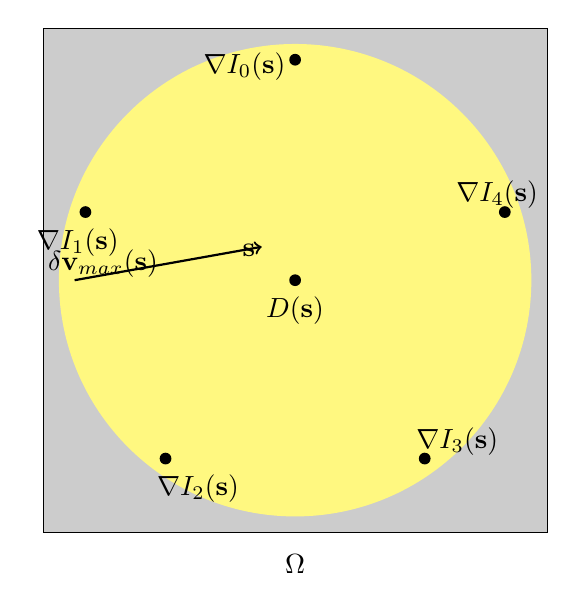
\begin{tikzpicture}[scale=0.8]

        % Define the square boundary of the image domain Ω
        \draw[fill=black!20] (-4,-4) rectangle (4,4);

        % Define the circle D(s)
        \node[circle, fill=yellow!50, minimum size=6cm] at (0,0) {};

        % Define the point s
        \node[above left=0.3cm and 0.5cm of {(0,0)}, inner sep=0pt, anchor=south east] (s) {$\mathbf{s}$};
        
        % Draw the gradients and their labels
        \foreach \i in {0,1,2,3,4} {
            \pgfmathsetmacro{\angle}{90 + 360/5 * \i}
            \node at (\angle:3.5cm) [circle,fill,inner sep=1.5pt,label={[anchor=\angle-90]below:$\nabla I_\i(\mathbf{s})$}] {};
        }

        % Draw the δv_max(s) vector connection
        \draw[->, thick] (180:3.5cm) -- node[left] {$\delta\mathbf{v}_{\text{max}}(\mathbf{s})$} (135:0.75cm);
        
        % Mark the center of the circle with a dot to indicate D(s)
        \node at (0,0) [circle,fill,inner sep=1.5pt,label=below:$D(\mathbf{s})$] {};

        % Label the image domain Ω
        \node at (0,-4.5) {$\Omega$};

    \end{tikzpicture}
    \caption{A diagram of the region \(D(\mathbf{s})\) in the image domain \(\Omega\). The individual gradients \(\nabla I_i(\mathbf{s})\) represent observations of the underlying gradient of the image surface \(\nabla I(\mathbf{s})\). For the local linearization to hold between \(I_0\) and \(I_2\), the gradient must be constant along the dotted line connecting these points. To check the validity of the linearization, consider gradients \(\nabla I_0(\mathbf{s})\), \(\nabla I_1(\mathbf{s})\), and \(\nabla I_2(\mathbf{s})\). If any of these gradients differ, the linearization is invalid.}
    \label{fig:image_domain}
\end{figure}

\end{document}